% copyright 2020 Edmundo Carmona Antoranz
% Released under the terms of Creative Commons Attribution-ShareAlike 4.0 International Public License

\section{Conflictos de archivo completo}

Así que, han disfrutado de los conflictos previos, cierto? Por supuesto! Bien... si les gustaron los anteriores, este lo van a {\bf amar}!

\subsection{Ejemplo 17}

Desde el \hyperref[openjdk_repo]{Repo del JDK de OpenJDK}, hagan checkout de la revisión {\bf 9d3e0870754} y mezclen {\bf 2978ffb9f9d}
\footnote{estos son los padres de la revisión {\bf e005d5df51e}}.

Verán que habrá un conflicto en el archivo {\bf langtools/src/share/classes/com/sun/tools/doclets/internal/toolkit/resources/doclet.xml}.
Pero no es solo {\it un} conflicto. Es {\bf el} conflicto. En vez de tener algunas líneas con conflicto, dentro del archivo,
todo el archivo está en conflicto. Aquí hay algunas líneas del archivo (los números de las líneas están a la izquierda):

\begin{lstlisting}[style=console_style,
	basicstyle=\small,
	caption={\bf Ejemplo 17} - Archivo en conflicto]
     1  <<<<<<< HEAD
     2  <?xml version='1.0' encoding='utf-8'?>
     3  
     4  <!--
     5   Copyright 2003 Sun Microsystems, Inc.  All Rights Reserved.
.
.
.
   205      </SerializedForm>
   206  </Doclet>
   207  ||||||| 4ae52d7dc1e
   208  <?xml version='1.0' encoding='utf-8'?>
   209  
.
.
.
   411      </SerializedForm>
   412  </Doclet>
   413  =======
   414  <?xml version='1.0' encoding='utf-8'?>
   415  
   416  <!--
.
.
.
   616          <Footer/>
   617      </SerializedForm>
   618  </Doclet>
   619  >>>>>>> 2978ffb9f9d
\end{lstlisting}

Antes de entrar en detalles, déjenme mostrarles lo que sucedió en {\bf la otra rama} en términos de los cambios sobre este archivo:

\begin{lstlisting}[style=console_style,
	basicstyle=\small,
	caption={\bf Ejemplo 17} - Cambios sobre {\bf la otra rama}]
$ git diff HEAD...MERGE_HEAD -- langtools/src/share/classes/com/sun/tools/doclets/internal/toolkit/resources/doclet.xml
diff --git a/langtools/src/share/classes/com/sun/tools/doclets/internal/toolkit/resources/doclet.xml b/langtools/src/share/classes/com/sun/tools/doclets/internal/toolkit/resources/doclet.xml
index 8eaa2d77abc..29c473790e4 100644
--- a/langtools/src/share/classes/com/sun/tools/doclets/internal/toolkit/resources/doclet.xml
+++ b/langtools/src/share/classes/com/sun/tools/doclets/internal/toolkit/resources/doclet.xml
@@ -1,7 +1,7 @@
 <?xml version='1.0' encoding='utf-8'?>
 
 <!--
- Copyright 2003 Sun Microsystems, Inc.  All Rights Reserved.
+ Copyright 2003-2009 Sun Microsystems, Inc.  All Rights Reserved.^M
  DO NOT ALTER OR REMOVE COPYRIGHT NOTICES OR THIS FILE HEADER.
 
  This code is free software; you can redistribute it and/or modify it
\end{lstlisting}

Un simple cambio de una sola línea. La línea es diferente a lo que tenemos en {\bf HEAD}?

\begin{lstlisting}[style=console_style,
	basicstyle=\small,
	caption={\bf Ejemplo 17} - archivo como está en {\bf HEAD}]
$ git show HEAD:langtools/src/share/classes/com/sun/tools/doclets/internal/toolkit/resources/doclet.xml | head -n 5
<?xml version='1.0' encoding='utf-8'?>

<!--
 Copyright 2003 Sun Microsystems, Inc.  All Rights Reserved.
 DO NOT ALTER OR REMOVE COPYRIGHT NOTICES OR THIS FILE HEADER.
\end{lstlisting}

La línea se ve justamente como lo que fue removido en {\bf la otra rama}... Esto pareciera ser algo muy fácil, cierto? No debería haber
{\bf ningún} conflicto, en realidad. Qué pasó entonces? Hay una respuesta muy rápida pero... Por qué ahorrarnos el placer de una explicación
larga?

Los archivos de texto están hechos de {\bf líneas}. git considera las líneas separadas que conforman un archivo para saber {\bf cuales líneas}
son las mismas y cuales fueron modificadas cuando se va a mezclar código. Ahora bien, alguna vez se han preguntado cómo se define lo que es
{\bf una línea}? Cada línea está separada de la siguiente a través de un marcador que se llama {\bf Salto de Línea} ({\bf EOL}, por sus siglas
en inglés). Pero hay un pequeño problema. No hay uno ni dos sino {\bf tres}(!!!) formatos diferentes de marcadores de {\bf EOL} y cada uno
está asociado a un sistema operativo diferente.

\begin{itemize}
	\item {\bf Mac}: {\bf CR} ({\bf Carriage Return}, caracter {\bf 0x0d}, lo que normalmente tratamos como {\bf {\textbackslash}r}
	en lenguages de programación)
	\item {\bf NIX}: {\bf LF} ({\bf Line Feed}, caracter {\bf 0x0a}, lo que normalmente tratamos como {\bf {\textbackslash}n}
	en lenguages de programación)
	\item {\bf Windows}: {\bf CRLF} ({\bf Carriage Return} seguido de {\bf Line Feed}, caracteres {\bf 0x0d0a})
\end{itemize}

Aquí hay un pequeño archivo de texto con 3 formatos diferentes de {\bf EOL} para que vean como cambian los archivos a nivel binario:
\begin{figure}
	\centering
	\caption{{\bf Mac} EOL}
	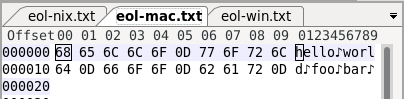
\includegraphics{eol-mac.png}
	\caption{{\bf NIX} EOL}
	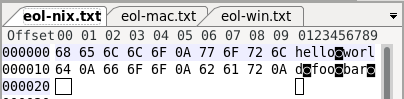
\includegraphics{eol-nix.png}
	\caption{{\bf Windows} EOL}
	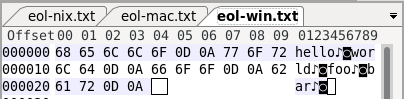
\includegraphics{eol-win.png}
\end{figure}

En un archivo nuevo, los editores de texto tienen la tendencia a colocar el formato de {\bf EOL} del sistema operativo sobre el que se está
trabajando. Si el archivo ya existía, los editores de texto\footnote{Por lo menos, los editores de texto {\bf decentes}} utilizan
el mismo formato del archivo, incluso si es diferente al sistema operativo sobre el que está trabajando el editor. Guarden un
archivo de texto en los diferentes formatos y vean como cambian los marcadores entre las líneas en un editor binario.

Podrían estarse preguntando ``Cómo terminamos en este desastre de {\bf EOL}?'' Es una pregunta apropiada y, justo como cualquier buena
historia, se trata de traiciones, puñaladas traperas de los amigos cercanos y ambición pero es algo que sale bastante del foco de este
manual así que les pediré amablemente que lean \href{https://es.wikipedia.org/wiki/Nueva_línea#Historia}{La Historia de la Nueva Línea}
si tienen curiosidad por saber como llegamos a este desastre.

Volviendo a nuestro problema particular, desde el punto de vusta de git, un cambio en el formato de {\bf EOL} efectivamente cambiará
el contenido de {\bf todas y cada una de las líneas} que conforman el archivo. Abren un arhivo, modifican una sola línea, guardan
cambiando el formato de {\bf EOL} y, para git, el archivo fue completamente limpiado y reescrito por completo.... en Esperanto. Es
un archivo completamente nuevo de cabo a rabo. Déjenme repetirlo para que el concepto cale: {\bf Archivo (pausa dramática) Completamente
(pausa dramática) Diferente}. Ninguna de las lineas preexistentes del archivo sobrevivió esa revisión.

Es este el caso de lo que pasó en este ejercicio? Pues veamos qué nos puede decir {\bf unix2dos} acerca del formato de {\bf EOL} del
archivo en las diferentes versiones involucradas:

\begin{lstlisting}[style=console_style,
	basicstyle=\small,
	caption={\bf Ejemplo 17} - tipos de {\bf EOL}]
$ git show HEAD:langtools/src/share/classes/com/sun/tools/doclets/internal/toolkit/resources/doclet.xml | unix2dos -imud
       0     205       0
$ git show MERGE_HEAD:langtools/src/share/classes/com/sun/tools/doclets/internal/toolkit/resources/doclet.xml | unix2dos -imud
     205       0       0
$ git show 4ae52d7dc1ef:langtools/src/share/classes/com/sun/tools/doclets/internal/toolkit/resources/doclet.xml | unix2dos -imud
     205       0       0
\end{lstlisting}

Y podemos ver cómo en {\bf HEAD} los saltos de línea están en una columna diferente, lo que indica un cambio de formato de {\bf EOL}.

Antes de entrar a considerar qué podemos hacer al respecto, preguntémonos ``{\bf Como fue que pasó esto en primer lugar?}'' Para nuestro
asombro, hay algunas posibilidades más o menos sencillas para que esto ocurra:

\begin{itemize}
	\item {\bf El desarrollador cambió el formato a propósito}. Podría haber una razón técnica para ello (Me es difícil pensar en
	una pero...) Pero si el cambio fue {\it solo por hacerlo}, esto merece un llamado de atención por toda la carga que este cambio
	genera más adelante (ya verán).
	
	\item {\bf El editor (IDE, editor de texto) lo cambió} sin que el desarrollador se de cuenta. Son cosas que pasan! Alguna vez han
	abierto un archivo NIX en el Notepad de Windows? Guardaron el archivo sin si quiera pensarlo? Ahí tienen!
	\footnote{Cuando se abre el archivo, se verá como si hubiera una sola línea muy larga dado que notepad no reconoce {\bf LF}
	como un salto de línea. Tiene que ser {\bf CRLF} porque {\it qué persona en su sano juicio podría pensar en utilizar algo que
	no sea software de Microsoft}, cierto? Por lo tanto, si guardan el archivo (si no se dan cuenta del problema y no salen corriendo),
	todos los saltos de línea desaparecerán. Y si decidieron separar todas las lineas del archivo {\it a pie} (Hey, no todos los
	desarrolladores están urgidos de hacer algo a la brevedad!), entonces todos los saltos de línea serán {\bf CRLF} en vez de los
	{\bf LF} originales. Y si esta crítica ya no es cierta porque hay un nuevo Microsoft Notepad que soporta diferentes formatos de
	{\bf EOL}, déjenme decirles que es {\bf ``excelente!''} Lástima que el cambio llegue con 30 años de retraso así que respaldo
	mi crítica.}
	Y apuesto a que hay otros editores que no mantienen el formato original de {\bf EOL}. De cualquier forma, este cambio de formato
	debió ser notado por el desarrollador {\bf antes} de publicar los cambios para que otros desarrolladores los halen dado que si
	otro desarrollador cambia dicho archivo y entonces hala (mezcla, hace rebase o cherry-pick) el cambio donde se cambia el
	formato de {\bf EOL}, van a terminar con un horrendo conflicto de archivo completo como los que estamos estudiando... {\it incluso
	si el cambio es de una sola línea}. Si usan un front-end decente para ver los cambios de las revisiones, deberían ver que incluso
	si lo que quisieron modificar fue una sola línea, todo el archivo se verá como que ha sido limpiado y vuelto a agregar de cabo
	a rabo. Ese es el síntoma que debería hacer que se den cuenta de que hay un problema y que deben corregirlo {\bf antes de publicar}.
	
	\item {el propio git se mete en el medio}. git tiene algunos trucos que pueden ser utilizados para configurar el formato
	de {\bf EOL} de los archivos. Personalmente, considero que son bastante difíciles de configurar apropiadamente considerando
	los diferentes sistema operativos, IDEs, etc. Siempre recomiendo configurar git para que no modifique los saltos de línea y dejar
	que los desarrolladores se hagan cargo. Y esto se puede lograr con un pequeño ajuste en el archivo {\bf .gitattributes} de tal
	forma que puede ser compartido por cualquiera que trabaje en un proyecto. Y si están totalmente seguros de que quieren dejar que
	git se encargue del formato de {\bf EOL}, asegúrense de leer los detalles al respecto comenzando con {\bf git help attributes},
	específicamente la sección relacionada a {\bf checking-out} y {\bf checking-in}. Esa es una muy buena lectura. Por último,
	pero no menos importante, no caigan en la trampa de usar {\bf core.autocrlf}. Lean de lo que se trata {\bf antes} de decidir
	qué valor utilizar allí\footnote{Si colocan el valor equivocado para core.crlf, tranquilamente podrían {\it dañar} muchos de los
	archivos del proyecto {\it sin si quiera haber abierto uno solo de ellos}.}
	
\end{itemize}

Ok, ok... suficiente teoría. Consideremos los diferentes enfoques que podrían seguir para salir de este enredo.

\subsection*{Quedarnos en HEAD, traer los cambios de la otra rama}

Lo primero que hay que notar es que esto está rompiendo bastante el objetivo de hacer un merge, cierto? Lo que quieren es que
todos los cambios de {\bf la otra rama} sean copiados {\it automágicamente} a su código y obtener conflictos en las secciones
que efectivamente lo sean. Ahora estamos en una situación donde tendremos que hacer todo {\bf a mano}. Afortunadamente, en este caso,
ya sabemos lo que se requiere que traigamos de {\bf la otra rama}. Tenemos que ajustar los años cubiertos por el copyright.
Por lo tanto, este sería el archivo resultante, las primeras líneas:

\begin{lstlisting}[style=xml_style,
	basicstyle=\small,
	caption={\bf Ejemplo 17} - {\bf HEAD} con los cambios de {\bf la otra rama}]
<<<<<<< HEAD
<?xml version='1.0' encoding='utf-8'?>

<!--
 Copyright 2003-2009 Sun Microsystems, Inc.  All Rights Reserved.
 DO NOT ALTER OR REMOVE COPYRIGHT NOTICES OR THIS FILE HEADER.
\end{lstlisting}

Removemos las otras partes del conflicto y los marcadores. Luego completamos el merge:

\begin{lstlisting}[style=console_style,
	basicstyle=\small,
	caption={\bf Ejemplo 17} - completar el {\bf merge}]
$ git add langtools/src/share/classes/com/sun/tools/doclets/internal/toolkit/resources/doclet.xml
$ git merge --continue
[detached HEAD b4a035c194c] Merge commit '2978ffb9f9d' into HEAD
\end{lstlisting}

Eso está bien. Como un arreglo rápido, esto hace el trabajo... {\bf pero} no hemos resuelto la verdadera {\bf causa del problema}.
Todavía hay una discrepancia en el {\bf formato de EOL} entre las ramas. Como un pequeño experimento, hagamos checkout de la rama que
acabamos de mezclar, {\bf 2978ffb9f9d}, escribamos un pequeño cambio sobre el archivo, regresemos a la revisión que acabamos de crear de mezcla
y pidamos mezclar de nuevo:

\begin{lstlisting}[style=console_style,
	basicstyle=\small,
	caption={\bf Ejemplo 17} - checkout {\bf 2978ffb9f9d}]
$ git checkout 2978ffb9f9d
Warning: you are leaving 1 commit behind, not connected to
any of your branches:

  b4a035c194c Merge commit '2978ffb9f9d' into HEAD

If you want to keep it by creating a new branch, this may be a good time
to do so with:

 git branch <new-branch-name> b4a035c194c

HEAD is now at 2978ffb9f9d Merge
\end{lstlisting}

Coloquemos que el copyright es 2003-2020, ahora, para los efectos de ejemplo\footnote{No tengo la intención de estar escribiendo
nada que sea legalmente vinculante, por si acaso}:

\begin{lstlisting}[style=xml_style,
	basicstyle=\small,
	caption={\bf Ejemplo 17} - Modificación sobre {\bf 2978ffb9f9d}]
<?xml version='1.0' encoding='utf-8'?>

<!--
 Copyright 2003-2020 Sun Microsystems, Inc.  All Rights Reserved.
 DO NOT ALTER OR REMOVE COPYRIGHT NOTICES OR THIS FILE HEADER.
\end{lstlisting}

Completamos la revisión:

\begin{lstlisting}[style=console_style,
	basicstyle=\small,
	caption={\bf Ejemplo 17} -  creando una nueva revisión]
$ git add langtools/src/share/classes/com/sun/tools/doclets/internal/toolkit/resources/doclet.xml
$ git commit -m "A tiny change"
[detached HEAD 0d57690bf36] A tiny change
 1 file changed, 1 insertion(+), 1 deletion(-)
\end{lstlisting}

En este punto, las dos revisiones que queremos mezclar se deben ver así (miren las dos revisiones superiores):
\begin{lstlisting}[style=console_style,
	basicstyle=\small,
	caption={\bf Ejemplo 17} - historia de las revisiones]
* 0d57690bf36 A tiny change
| *   b4a035c194c Merge commit '2978ffb9f9d' into HEAD
| |\  
| |/  
|/|   
* | 2978ffb9f9d Merge
| * 9d3e0870754 Merge
|/  
* 4ae52d7dc1e Added tag jdk7-b50 for changeset 7faffd237305
\end{lstlisting}

Intentemos mezclar de nuevo:

\begin{lstlisting}[style=console_style,
	basicstyle=\small,
	caption={\bf Ejemplo 17} - nueva mezcla]
$ git checkout b4a035c194c
Warning: you are leaving 1 commit behind, not connected to
any of your branches:

  0d57690bf36 A tiny change

If you want to keep it by creating a new branch, this may be a good time
to do so with:

 git branch <new-branch-name> 0d57690bf36

HEAD is now at b4a035c194c Merge commit '2978ffb9f9d' into HEAD
$ git merge 0d57690bf36
Auto-merging langtools/src/share/classes/com/sun/tools/doclets/internal/toolkit/resources/doclet.xml
CONFLICT (content): Merge conflict in langtools/src/share/classes/com/sun/tools/doclets/internal/toolkit/resources/doclet.xml
Automatic merge failed; fix conflicts and then commit the result.
\end{lstlisting}

Pues, tenemos un conflicto. Y al mirar dentro, será un conflicto de archivo completo {\bf de nuevo}:

\begin{lstlisting}[style=console_style,
	basicstyle=\small,
	caption={\bf Ejemplo 17} - archivo con conflicto... {\bf de nuevo}]
     1  <<<<<<< HEAD
     2  <?xml version='1.0' encoding='utf-8'?>
     3  
     4  <!--
     5   Copyright 2003-2009 Sun Microsystems, Inc.  All Rights Reserved.
     6   DO NOT ALTER OR REMOVE COPYRIGHT NOTICES OR THIS FILE HEADER.
.
.
.
   205      </SerializedForm>
   206  </Doclet>
   207  ||||||| 2978ffb9f9d
   208  <?xml version='1.0' encoding='utf-8'?>
   209  
   210  <!--
   211   Copyright 2003-2009 Sun Microsystems, Inc.  All Rights Reserved.
   212   DO NOT ALTER OR REMOVE COPYRIGHT NOTICES OR THIS FILE HEADER.
.
.
.
   411      </SerializedForm>
   412  </Doclet>
   413  =======
   414  <?xml version='1.0' encoding='utf-8'?>
   415  
   416  <!--
   417   Copyright 2003-2020 Sun Microsystems, Inc.  All Rights Reserved.
   418   DO NOT ALTER OR REMOVE COPYRIGHT NOTICES OR THIS FILE HEADER.
.
.
.
   617      </SerializedForm>
   618  </Doclet>
   619  >>>>>>> 0d57690bf36
\end{lstlisting}

No les estoy tomando el pelo. Mientras haya diferentes formatos de {\bf EOL} entre las ramas involucradas en un {\bf merge}... o {\bf rebase}...
o {\bf cherry-pick}... o {\bf revert}, van a ver estos conflictos totalmente inútiles... {\bf todas}... {\bf y cada una}... {\bf de las veces}.

Consideren que, en este caso, era un cambio un pequeño que tuvo que ser movido desde {\bf la otra rama}. Pero y si fueran cambios
mas grandes? Multiples cambios? Unos cambios que no deberían dar conflicto y algunos que si deberían generar conflicto? Están
dispuestos a pasar copiando cosas de un lado al otro todo el día? No es la mejor forma de gastar ciclos de CPU de nuestro
cerebro duramente entrenado para hacer mezclas, cierto? Exacto, lo mismo pensé.

Dado que, en nuestro ejemplo, el cambio de formato de {\bf EOL} sucedió en {\bf nuestra} rama, deberíamos cambiar el formato de {\bf EOL}
de vuelta al original antes de intentar hacer el {\bf merge}? Eso podría funcionar. Veamos. Primero, comencemos de nuevo:

\subsection{Ejemplo 17 - de nuevo... con un giro}

Desde el \hyperref[openjdk_repo]{repositorio JDK de OpenJDK}, hagan checkout de la revisión {\bf 9d3e0870754}. Abran el archivo
y cambien el formato de {\bf EOL} a Windows\footnote{Cualquier editor de texto {\it decente} les debe permitir hacer el cambio. Yo
voy a usar {\bf unix2dos}}. Luego acometan. Luego mezclen {\bf 2978ffb9f9d}.

\begin{lstlisting}[style=console_style,
	basicstyle=\small,
	caption={\bf Ejemplo 17} - intentando el {\bf merge} de nuevo]
$ git checkout 9d3e0870754
HEAD is now at 9d3e0870754 Merge
$ unix2dos langtools/src/share/classes/com/sun/tools/doclets/internal/toolkit/resources/doclet.xml
unix2dos: converting file langtools/src/share/classes/com/sun/tools/doclets/internal/toolkit/resources/doclet.xml to DOS format...
$ git add langtools/src/share/classes/com/sun/tools/doclets/internal/toolkit/resources/doclet.xml
$ git commit -m "Changing EOL-format"
[detached HEAD d5bb2068164] Changing EOL-format
 1 file changed, 205 insertions(+), 205 deletions(-)
$ git merge 2978ffb9f9d
Auto-merging langtools/src/share/classes/com/sun/tools/javac/util/RawDiagnosticFormatter.java
Auto-merging langtools/src/share/classes/com/sun/tools/javac/util/BasicDiagnosticFormatter.java
Auto-merging langtools/src/share/classes/com/sun/tools/javac/util/AbstractDiagnosticFormatter.java
Auto-merging langtools/src/share/classes/com/sun/tools/javac/resources/compiler.properties
.
.
.
 langtools/test/tools/javac/processing/model/testgetallmembers/Main.java                                | 2 +-
 langtools/test/tools/javadoc/6176978/T6176978.java                                                     | 2 +-
 langtools/test/tools/javadoc/6176978/X.java                                                            | 2 +-
 83 files changed, 83 insertions(+), 83 deletions(-)
$
\end{lstlisting}

Y esta vez el {\bf merge} no tuvo problemas. {\bf Somos tan buenos}. No está especificado en esa salida de la consola
pero la revisión del merge es {\bf cddf9316c72}. Así que esto es lo que tuvimos que hacer desde el principio, cierto?
Hacer que ambas ramas tengan el mismo formato de {\bf EOL} de {\bf el ancestro común} y entonces mezclar. Bueno, sí,
eso {\bf funciona}. Pudieron mezclar (incluso mejor, no hubo conflictos!). Pero, como un giro adicional, hagamos un checkout
de la revisión original desde la que comenzamos a trabajar, {\bf 9d3e0870754}, modifiquemos una línea del archivo, un cambio
inocente, creemos una revisión, regresemos a la revisión de merge que acabamos de crear e intentemos mezclar de nuevo, bien?
Qué creen que va a pasar?

\begin{lstlisting}[style=console_style,
	basicstyle=\small,
	caption={\bf Ejemplo 17} - checkout de {\bf 9d3e0870754}]
$ git checkout 9d3e0870754
HEAD is now at 9d3e0870754 Merge
\end{lstlisting}

\begin{lstlisting}[style=xml_style,
	basicstyle=\small,
	caption={\bf Ejemplo 17} - Modificando el archivo sobre {\bf 9d3e0870754}]
<?xml version='1.0' encoding='utf-8'?>


<!--
 Copyright 2003 Sun Microsystems, Inc.  All Rights Reserved.
 DO NOT ALTER OR REMOVE COPYRIGHT NOTICES OR THIS FILE HEADER.
\end{lstlisting}

Agregué una segunda línea vacía antes del comentario XML.

\begin{lstlisting}[style=console_style,
	basicstyle=\small,
	caption={\bf Ejemplo 17} - completando la revisión]
$ git add langtools/src/share/classes/com/sun/tools/doclets/internal/toolkit/resources/doclet.xml
$ git commit -m "Adding empty line"
[detached HEAD 91df2b0b521] Adding empty line
 1 file changed, 1 insertion(+)
\end{lstlisting}

Como se ve la historia en este momento?

\begin{lstlisting}[style=console_style,
	basicstyle=\small,
	caption={\bf Ejemplo 17} - historia actual]
* 91df2b0b521 Adding empty line
| *   cddf9316c72 Merge commit '2978ffb9f9d' into HEAD
| |\  
| | *   2978ffb9f9d Merge
| | |\  
| | * | 56fcf6c0524 6814575: Update copyright year
| * | | d5bb2068164 Changing EOL-format
|/ / /  
* | |   9d3e0870754 Merge
\end{lstlisting}

Ahora hagamos checkout de {\bf cddf9316c72} y tratemos de mezclar la revisión que acabamos de crear.

\begin{lstlisting}[style=console_style,
	basicstyle=\small,
	caption={\bf Ejemplo 17} - Mezclando de nuevo]
$ git checkout cddf9316c72
Warning: you are leaving 1 commit behind, not connected to
any of your branches:

  91df2b0b521 Adding empty line

If you want to keep it by creating a new branch, this may be a good time
to do so with:

 git branch <new-branch-name> 91df2b0b521

HEAD is now at cddf9316c72 Merge commit '2978ffb9f9d' into HEAD
$ git merge 91df2b0b521
Auto-merging langtools/src/share/classes/com/sun/tools/doclets/internal/toolkit/resources/doclet.xml
CONFLICT (content): Merge conflict in langtools/src/share/classes/com/sun/tools/doclets/internal/toolkit/resources/doclet.xml
Automatic merge failed; fix conflicts and then commit the result.
\end{lstlisting}

Y apuesto a que esta vez tienen una idea del tamaño de este conflicto, me equivoco? Y si no lo saben, aquí les doy una pista: Comienza con
{\bf conflicto} y termina en {\bf de archivo completo}. Y pueden ver como al mezclar una rama que fue arrancada antes de corregir el
formato de {\bf EOL} a lo que era originalmente, nos volvemos a conseguir con nuestro desastre.

Pero entonces como se sale de este desastre? El mejor enfoque que podrían tomar es reescribir la historia para que el cambio de
formato de {\bf EOL} no ocurra. Yo se, yo se.... no es {\bf recomendado como principio general}, pero hay situaciones que lo ameritan.
Yo diría que esta es una de esas situaciones. En la sección de \hyperref[recipes]{Recetas}, incluí una forma más o menos
sencilla de reescribir la historia de una rama {\it siempre y cuando sea recta, es decir, no tenga merges}.
 
Si reescribir la historia no es una opción, entonces ajusten el formato de {\bf EOL} al original en la rama en la que fue cambiado
y carguen con las consecuencias. Desafortunadamente están manejando una situación que no debió suceder en primer lugar. Si un desarrollador
cambia el formato de {\bf EOL} de un archivo en un PR, eso nunca debió ser aceptado. Debió ser rechazado, el desarrollador debió coregir la
historia de la rama tal que el cambio de formato nunca sucede (la rama puede ser corregida con muy poco esfuerzo usando la receta, ok?).

\subsection{Ejercicios}
\subsubsection{Ejercicio 8 - usando el script}
 
Del \hyperref[exercises_repo]{repo de ejercicios}, hagan checkout de la rama {\bf exercise8/branchA} y hagan merge de {\bf exercise8/branchB}.
Deberíamos ver un conflicto de archivo completo en {\bf primes.py}.

Traten de hacer el {\bf merge} corrigiendo la historia de la rama usando el script dado en \hyperref[correct_eol_history]{esta receta}.
La solución está \hyperref[exercise08]{aquí}.

\subsection{Tips}
\begin{itemize}
	\item Asegúrense de que los archivos nunca cambian su formato de {\bf EOL}... {\it a menos que sea {\bf verdaderamente} requerido}.
	\item Si un archivo tuvo un cambio de formato de{\bf EOL} (sin una razón legítima), {\bf no acepten ese cambio}.
	\item Usen el script descrito \hyperref[correct_eol_history]{aquí} para corregir la historia de la rama si notan que hubo un cambio
	de formato de {\bf EOL} antes de mezclarlo en otras ramas.
	\item Asegúrense de que sus herramientas estén configuradas para {\bf no} ocultar cambios de {\bf EOL}.
\end{itemize}
